\section{Velvet Interlinks}
\subsection{Velvet fork parameter}
In a velvet fork, only a minority of honest parties needs to support the protocol
changes. We refer to this percentage as the ``velvet parameter''.

\begin{definition}[Velvet Parameter]
	The \emph{velvet parameter} $g$ is defined as the percentage of honest parties
	that have upgraded to the new protocol. The absolute number of honest upgraded
	parties is denoted $n_h$ and it holds that
	$n_h = g (n - t)$.
	\label{defn:velvet_honest_majority}
\end{definition}

\subsection{Smooth and Thorny blocks}
In order to be applied under velvet fork, a protocol has to change in a backwards-compatible manner. In essence, any additional information coming with the protocol upgrade is transparent to the non-upgraded players. This transparency towards the non-upgraded parties requires any block that conforms only to the old protocol rules to be considered a valid one. Considering superblock NIPoPoWs under a velvet fork, any block is to be checked for its validity regardless the validity of the NIPoPoWs protocol's additional information, which is the interlink structure.

A block generated by the adversary could thus contain arbitrary data in the interlink and yet be appended in the chain adopted by an honest party. In case that trash data are stored in the structure this could be of no harm for the protocol routines, since such blocks will be treated as non-upgraded. In the context of the attack that will be presented in the following section, we examine the case where the adversary includes false interlink pointers.

An interlink pointer is the hash of a block. A correct interlink pointer of a block $b$ for a specific level $\mu$ is a pointer to the most recent $b$'s ancestor of level $\mu$. From now on we will refer to correct interlink pointers as \emph{smooth pointers}. Pointers of the 0-level \textit{(prevIds)} are always smooth because of the performed proof-of-work.

\begin{definition}[Smooth Pointer]
  Smooth pointer of a block $b$ for a specific level $\mu$ is the     interlink pointer to the most recent $\mu$-level ancestor of $b$.
	\label{defn:smooth_pointer}
\end{definition}


A non-smooth pointer may not point to the most recent ancestor of level $\mu$ or even point to a superblock of a fork chain, as shown in Figure \ref{fig:false_interlink}.

\begin{figure}[h]
	\begin{center}
		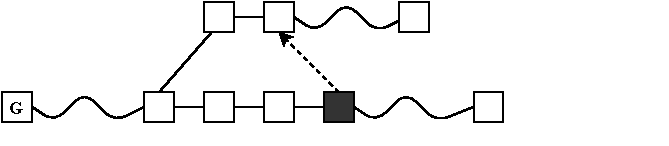
\includegraphics[scale=0.7]{figures/false_interlink.pdf}
	\end{center}
    \caption{A non-smooth pointer of an adversarial block, colored  black, in an honest player's chain.}
	\label{fig:false_interlink}
\end{figure}

In the same manner it is possible that a false interlink contain arbitrary pointers to blocks of any chain as illustrated in Figure \ref{fig:thorny_block}. The interlink pointing to arbitrary directions resembles a thorny bush, so we will refer to blocks containing false interlink information as \emph{thorny}.

\begin{definition}[Thorny Block]
	Thorny block is a block which contains at least one non-smooth interlink pointer.
	\label{defn:thorny_block}
\end{definition}

\begin{figure}[h]
	\begin{center}
		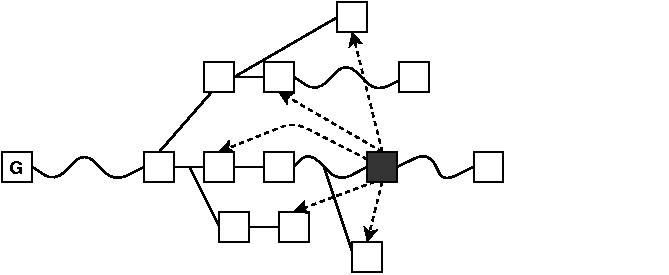
\includegraphics[scale=0.75]{figures/thorny_block.pdf}
	\end{center}
	\caption{A thorny block appended in an honest player's chain.
	The dashed arrows are interlink pointers.}
	\label{fig:thorny_block}
\end{figure}

Opposite of the thorny are the \emph{smooth} blocks, which may be blocks generated by non-upgraded players or blocks generated by upgraded players and contain only smooth pointers in their interlink.

\begin{definition}[Smooth Block]
	Smooth block is any block which is not thorny.
	\label{defn:smooth_block}
\end{definition}
